%
% File acl2014.tex
%
% Contact: koller@ling.uni-potsdam.de, yusuke@nii.ac.jp
%%
%% Based on the style files for ACL-2013, which were, in turn,
%% Based on the style files for ACL-2012, which were, in turn,
%% based on the style files for ACL-2011, which were, in turn,
%% based on the style files for ACL-2010, which were, in turn,
%% based on the style files for ACL-IJCNLP-2009, which were, in turn,
%% based on the style files for EACL-2009 and IJCNLP-2008...

%% Based on the style files for EACL 2006 by
%%e.agirre@ehu.es or Sergi.Balari@uab.es
%% and that of ACL 08 by Joakim Nivre and Noah Smith

\documentclass[11pt]{article}
\usepackage{acl2014}
\usepackage{times}
\usepackage{url}
\usepackage{latexsym}
\usepackage[backend=bibtex]{biblatex}
\usepackage{graphicx}
\addbibresource{citations}


%\setlength\titlebox{5cm}

% You can expand the titlebox if you need extra space
% to show all the authors. Please do not make the titlebox
% smaller than 5cm (the original size); we will check this
% in the camera-ready version and ask you to change it back.


\title{MIM QA System: Deliverable 3}

\author{Antariksh Bothale \\
  {\tt abothale@uw.edu} \\\And
  Julian Chan\\
  {\tt jchan3@uw.edu} \\\And
  Yi-shu Wei\\
  {\tt yishuwei@uw.edu}}

\date{}

\begin{document}
\maketitle
\begin{abstract}
We detail the work currently done on MIM, our Question Answering system. We report a lenient MRR score of 0.3609 (strict score 0.2433), and detail the improvements made in the system to achieve said score.
\end{abstract}

\section{Introduction}
This document reports the creation and performance of an end-to-end Question Answering system. We have a basic setup in place for the overall task and present current baseline results.

\section{System Overview}

Our system architecture can be broken down into three major classes - MainFacilitator, TaskExecutor, and Session. Our information retrieval system processes queries and retrieves answers in 5 steps, namely Question Classification, Query Formation, Document Retrieval, Passage Retrieval, and Answer Processing. Each of these steps are encapsulated in their own class and derives from the TaskExecutor task.  The Session object is used to pass information between these tasks. The implementation of each TaskExecutor is completely transparent to the MainFacilitator, whose job is to simply run the TaskExecutor(s) in the correct order and pass a Session object between them. The QuestionProcessor object is embedded in the Session object and contains methods that allows the TaskExecutor(s) to access the user query.

During start-up, MainFacilitator instantiates the five TaskExecutor(s) and put them in an array. When there is a new query and the AnswerQuestion() method is called, MainFacilitator creates a new Session object and calls Execute() on each of the TaskExecutor(s) sequentially. Barring any execution error, the answer will be written to the Session object.

The SystemEvaluator reads in all the question from the data set and calls MainFacilitator's AnswerQuestion() function. It then reads the answer from the returned Session object and
writes to the output file.

%\begin{figure*}
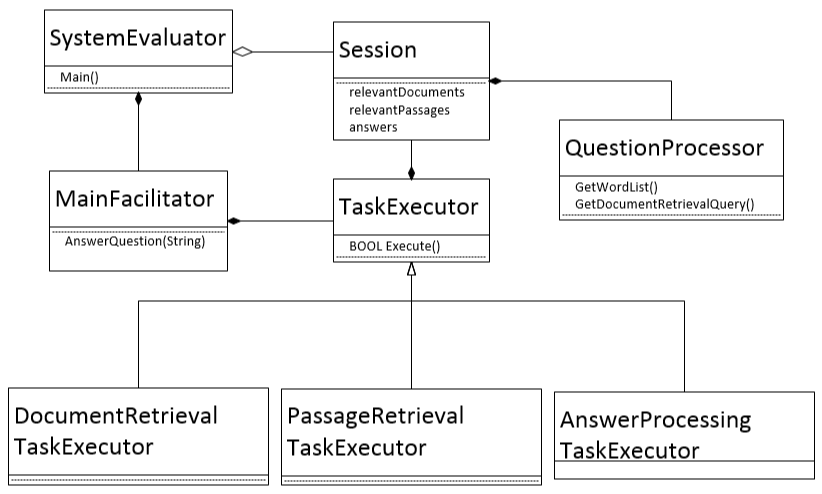
\includegraphics[width=3in,height=1.75in]{MIM_class_diagram.png}
Fig 1: class diagram of the MIM QA system
%\end{figure*}


\section{Approach}
\subsection{Question Classification}
We build an SVM classifier that classifies a given question into one of the question types defined in the UIUC question taxonomy \cite{uiuc}. The classifier uses unigrams as well as the {\it Wh-} words and the headwords as features. (Headwords are extracted from parsing the questions using the Berkeley parser \cite{berkeleyparser}).

We train the classifier on the dataset from \cite{uiuc} with 5500 labeled questions, and test the classifier on TREC 2004 and 2005 question-answering data. Since the test data are only labeled for coarse-grained question types (6 classes), we can only evaluate the classifier with coarse-grained classification, for which our SVM classifier achieves 87\% accuracy. However, for our end-to-end system we retrained the classifier for fine-grained question classification (50 classes) because coarse-grained class label does not provide sufficient information for selecting correct answers.

\subsection{Query Formation by Redundancy-based Web-boosting}
In this step we convert the question into a query that can be used for document retrieval. The query indicates that the subsequent module should search for the question terms (except the {\it Wh-} words) in the body text, and for the target words either in the title or the body text.

We implemented query expansion using a redundancy-based web-boosting strategy. The original question (together with the target words) is passed to the Ask.com search engine and the snippets of the first 40 results are extracted. From these snippets we obtain bigram counts and keep only the top 10 most frequent ones that do not contain any words from the original question. Often times, we found these top bigrams to  contain the correct answer to the questions.

We then harvest unique terms from these top bigrams and add them to the query to the document retrieval system. We were able to increase our accuracy significantly (at least 10 points).

\subsection{Document Retrieval}
The Document Retrieval Subsystem takes a document retrieval query from the session and populates the session with a list of hits from the indexing and retrieval system, as described below. This list of documents is then used for Passage Retrieval and Answer Processing.

For the purpose of indexing and searching the documents, we use Whoosh \cite{whoosh}, which is pure-Python based text indexing, search, and spell checking library. The choice of a Python based library above alternatives such as Lucene and Indri/Lemur was motivated by its ease of integration and use with our Python code-base, and its functionality being comparable to that of its Java counterparts.

\subsubsection{Indexing}
The Beautiful Soup XML parser \cite{bsoup} was used to parse all the documents and extract the Document ID, Headline and Body Text. Whoosh's in-built indexing engine was used to index all the documents present in the corpus. The current system uses Whoosh's default indexing mechanism, which does not process the text, we plan to improve on this by incorporating tokenization and stemming. The indexing schema was designed to store the Document ID and Headline with the Index, while the Body Text was indexed but not stored as it would have caused unnecessary duplication of data. Instead, the text is retrieved from the document using the Document ID whenever needed. This index is currently stored on Patas.

\subsection{Passage Retrieval}
This step reads the files retrieved in the last step, extracting all passages in the documents that contain the keywords (the target words, the words in the question, and the words added from web-boosting). A ``passage'' in our current system is simply defined as a sentence, where sentence segmentation is handled by Whoosh. These passages are then scored based on the density of keywords in the passage. The passage extraction and scoring function are taken from Whoosh, which are originally used for returning snippets for search results.

\subsection{Answer Processing}
We do re-ranking based on pattern matching, and then chop off anything after 250 characters. If the question is classified to be of type \emph{HUM}, any answer with named entities of type \emph{PERSON} (as classified by NLTK) are bumped above answers without such entities. Likewise, for questions of type \emph{NUM:date}, answers that have a pattern match with a date / year pattern are bumped up. Finally, for questions of type \emph{NUM}, we prioritize answers with numerical patterns in them. If there are multiple answers that satisfy any of the above criteria, we do not break ties between them and return them in the relative order in which they were returned by the passage retrieval system.

\section{Results}

Under the baseline system, we obtain an aggregate score of 0.2433 under the Strict evaluation scheme, and an aggregate score of 0.3609 under the Lenient evaluation scheme.

The big improvement from last deliverable comes from several sources: First, we include the target words in our query; second, we use the whole sentence rather than automatically generated snippets as our answers; third, we exploit search results from the World Wide Web and use question classification and relevant answer re-ranking.

\section{Discussion}
\label{sec:discussion}

The baseline system has been put in place and works end to end, but since it uses fairly naive and rudimentary processing methods at each step of the chain, the results are far from satisfactory. The next few weeks on the project would now be devoted to improving each of the segments.
\section*{Acknowledgments}
We thank C J Hsu for the code snippet for interfacing with Ask.com for the Web Boosting mode that he shared with all students on GoPost.

\printbibliography

\end{document}
